\documentclass[12pt,letterpaper]{article}
\usepackage[utf8]{inputenc}
\usepackage[T1]{fontenc}
\usepackage[spanish]{babel}
\usepackage{mathptmx}
\usepackage[margin=1in]{geometry}
\usepackage{setspace}
\usepackage{graphicx}
\setstretch{1.15}
\setlength{\parindent}{0pt}
\setlength{\parskip}{8pt}
\pagestyle{plain}
\newcommand{\titulo}[1]{\vspace{6pt}{\LARGE #1}\par\vspace{4pt}}
\newcommand{\subtitulo}[1]{\vspace{6pt}{\Large #1}\par}
\begin{document}

Luis Alberto Román Verde

\titulo{Análisis de una interacción social}

La interacción que elegí fue un día en que esperábamos al profesor de Óptica. Éramos seis personas en el salón. Como el profe suele llegar tarde, al principio nadie se preocupó y nos quedamos platicando y viendo el celular. Nadie intentó contactarlo. Después de casi media hora nos mandó un mensaje diciendo que ya no alcanzaba a llegar, y fue hasta entonces que nos fuimos. Yo no hice nada en particular, solo me quedé platicando con los demás.

Esta interacción sí responde a una norma social, que es la regla no escrita de esperar al profesor cierto tiempo antes de irse, que normalmente se dice que son 15 minutos. También funcionó otra norma más implícita, la de no ser el primero en irse, porque irte sin que el profesor diga algo se siente como una falta, aunque el que faltó fue él.

Lo extraño en lo familiar es que esperamos el doble de lo que dice esa regla y nadie se fue ni le escribió. Como ya estamos acostumbrados a que llegue tarde, lo vimos como algo normal. Pero si alguien de fuera viera la escena, le parecería raro que seis personas se queden media hora sentadas esperando a alguien sin saber si va a llegar, dejando que él decida por todos.

También hay desigualdad, porque la espera no afecta igual a todos. Mucha gente viene de lejos, por ejemplo una amiga mía viene desde Zapotlanejo, así que para ella esa media hora implica más tiempo y dinero invertidos en una clase que al final no hubo. Además, se nota una diferencia entre el tiempo del profesor y el de los alumnos, ya que si nosotros llegamos tarde hay consecuencias, pero si él llega tarde o no llega, no pasa nada.

Por último, sí hay un uso del poder. Lo interesante es que el profesor lo ejerció sin estar presente. Como él es quien pone las faltas y las calificaciones, su autoridad bastó para que nos quedáramos esperando, y al final fue su mensaje lo que decidió el momento en que nos íbamos. Es un poder que viene de su papel dentro de la universidad y no de algo que haya hecho ese día.

\newpage
\titulo{Mi ubicación social}

Soy hombre, tengo 21 años, soy de clase media alta, no tengo religión y estudio en el ITESO, que es una universidad privada. Rento un departamento atrás del ITESO y llego en carro, así que no tengo que hacer trayectos largos ni depender del transporte público. En ese sentido sí tengo algunas ventajas.

Aun así, siento que estoy bastante lejos de los centros de poder. No tengo dinero propio, dependo de mi familia para la renta y mis gastos, y no tengo influencia real en las decisiones importantes de la sociedad, como las que toman el gobierno o los grandes empresarios. Por eso me ubico en medio de la clase media, con algunas ventajas pero muy lejos de donde realmente se decide cómo funcionan las cosas.

Si me comparo con mi amiga que viene desde Zapotlanejo, ella estaría un poco más abajo que yo, aunque no mucho. Ella estudia en el CUCEI y todos los días tiene que hacer un trayecto mucho más largo que el mío, lo que significa más tiempo y más dinero solo para poder llegar a clases. Algo tan simple como vivir cerca o lejos de la escuela ya marca una diferencia en las oportunidades y el tiempo que cada quien tiene, y eso es parte de la ubicación social.

\subtitulo{Mapa social}
\begin{center}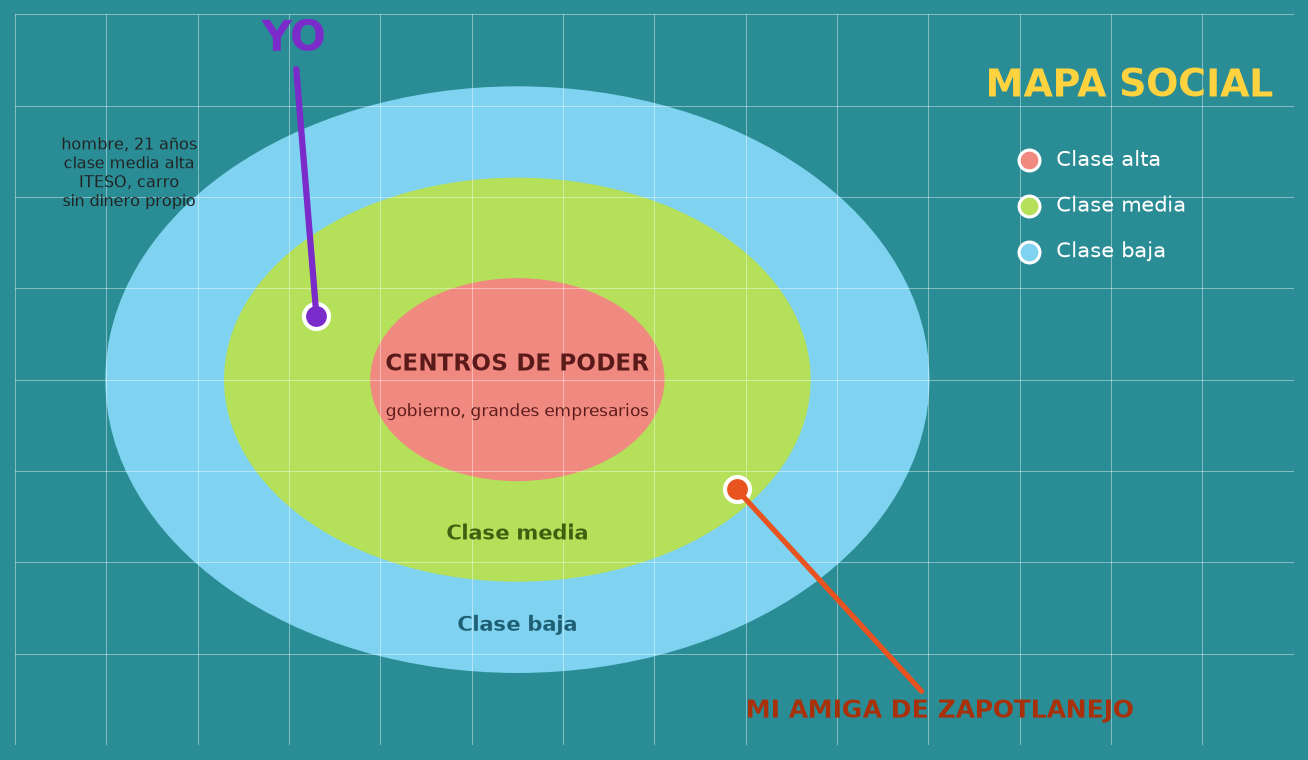
\includegraphics[width=\textwidth]{mapa_social.png}\end{center}

\newpage
\titulo{Mi concepto de desigualdad}

Para mí la desigualdad es cuando las personas no tienen las mismas oportunidades ni los mismos recursos, no por lo que hacen o por su esfuerzo, sino por el lugar en el que nacieron o en el que les tocó estar. Creo que en México donde más se nota es en lo económico. Hay una diferencia enorme entre lo que tienen unos pocos y lo que tiene la mayoría, y esa diferencia termina afectando casi todo lo demás, como la educación, la salud, el transporte o incluso el tiempo libre que tiene cada persona.

Pienso que esto se debe principalmente a la concentración de la riqueza y a las dinámicas de poder. Quienes tienen más dinero también suelen tener más influencia en las decisiones políticas y económicas, y eso les permite mantener su posición, mientras que a quienes tienen menos se les hace cada vez más difícil salir adelante. Es como un ciclo que se repite y se va heredando de una generación a otra.

\subtitulo{¿Cómo lo sé y dónde lo he observado?}

Esto lo sé principalmente por mi familia. Mis papás son doctores en economía, así que toda mi vida he escuchado conversaciones sobre la distribución del ingreso, la concentración de la riqueza y temas parecidos. Más que haberlo investigado por mi cuenta, es algo que fui aprendiendo en la casa casi sin darme cuenta.

Por lo mismo, creo que mi forma de ver la desigualdad tiene un sesgo. Como crecí escuchando sobre la desigualdad económica, es normal que sea lo primero que pienso cuando se habla del tema, y probablemente le doy menos importancia a otros tipos de desigualdad, como la de género, la racial o la regional. Aun así, también lo he observado en mi día a día, por ejemplo en la diferencia entre mi situación y la de mi amiga que viene desde Zapotlanejo, donde algo tan simple como el dinero y la distancia ya cambia mucho las oportunidades de cada quien.

\end{document}